\section{Methods}

First, both datasets were split in a class-disjoint way into two sets with a ratio of 7 to 3. The latter is the \textit{test} split while the former was further divided into \textit{train} (80\%) and \textit{evaluation} (20\%) splits.

For implementing the fine-tuning, training, and evaluation of the models, the following libraries were used: gensim \cite{vrehuuvrek2011gensim}, Hugging Face's transformers \cite{wolf2019huggingface}, PyTorch \cite{paszke2019pytorch}, and scikit-learn \cite{pedregosa2011scikit}.

\subsection{Steps}

The main idea of the compared methods is to fine-tune two distinct models on different (but semantically related) tasks and then analyse and utilise the hypothesised similarity in their embedding spaces. Figure \ref{fig:fine-tune} shows the fine-tuning stage. Each model (except TF-IDF\footnote{In the case of TF-IDF, no fine-tuning or classification task is required. It only needs the captions to create a dictionary and use it for mapping any textual input into a vector.}) has a fully-connected top layer with as many outputs as there are classes in the \textit{train} split. After fine-tuning, the embeddings of the \textit{train} dataset are also calculated and stored for later use.

For the image classification, the learning rate was \num{1e-3} and constant for all networks, crops and resizing were used for data augmentation. DistilBERT had a learning rate of \num{2e-5} and a weight decay of $0.01$ for regularisation. All networks used minibatches of size $32$.

\begin{figure}
  \centering
  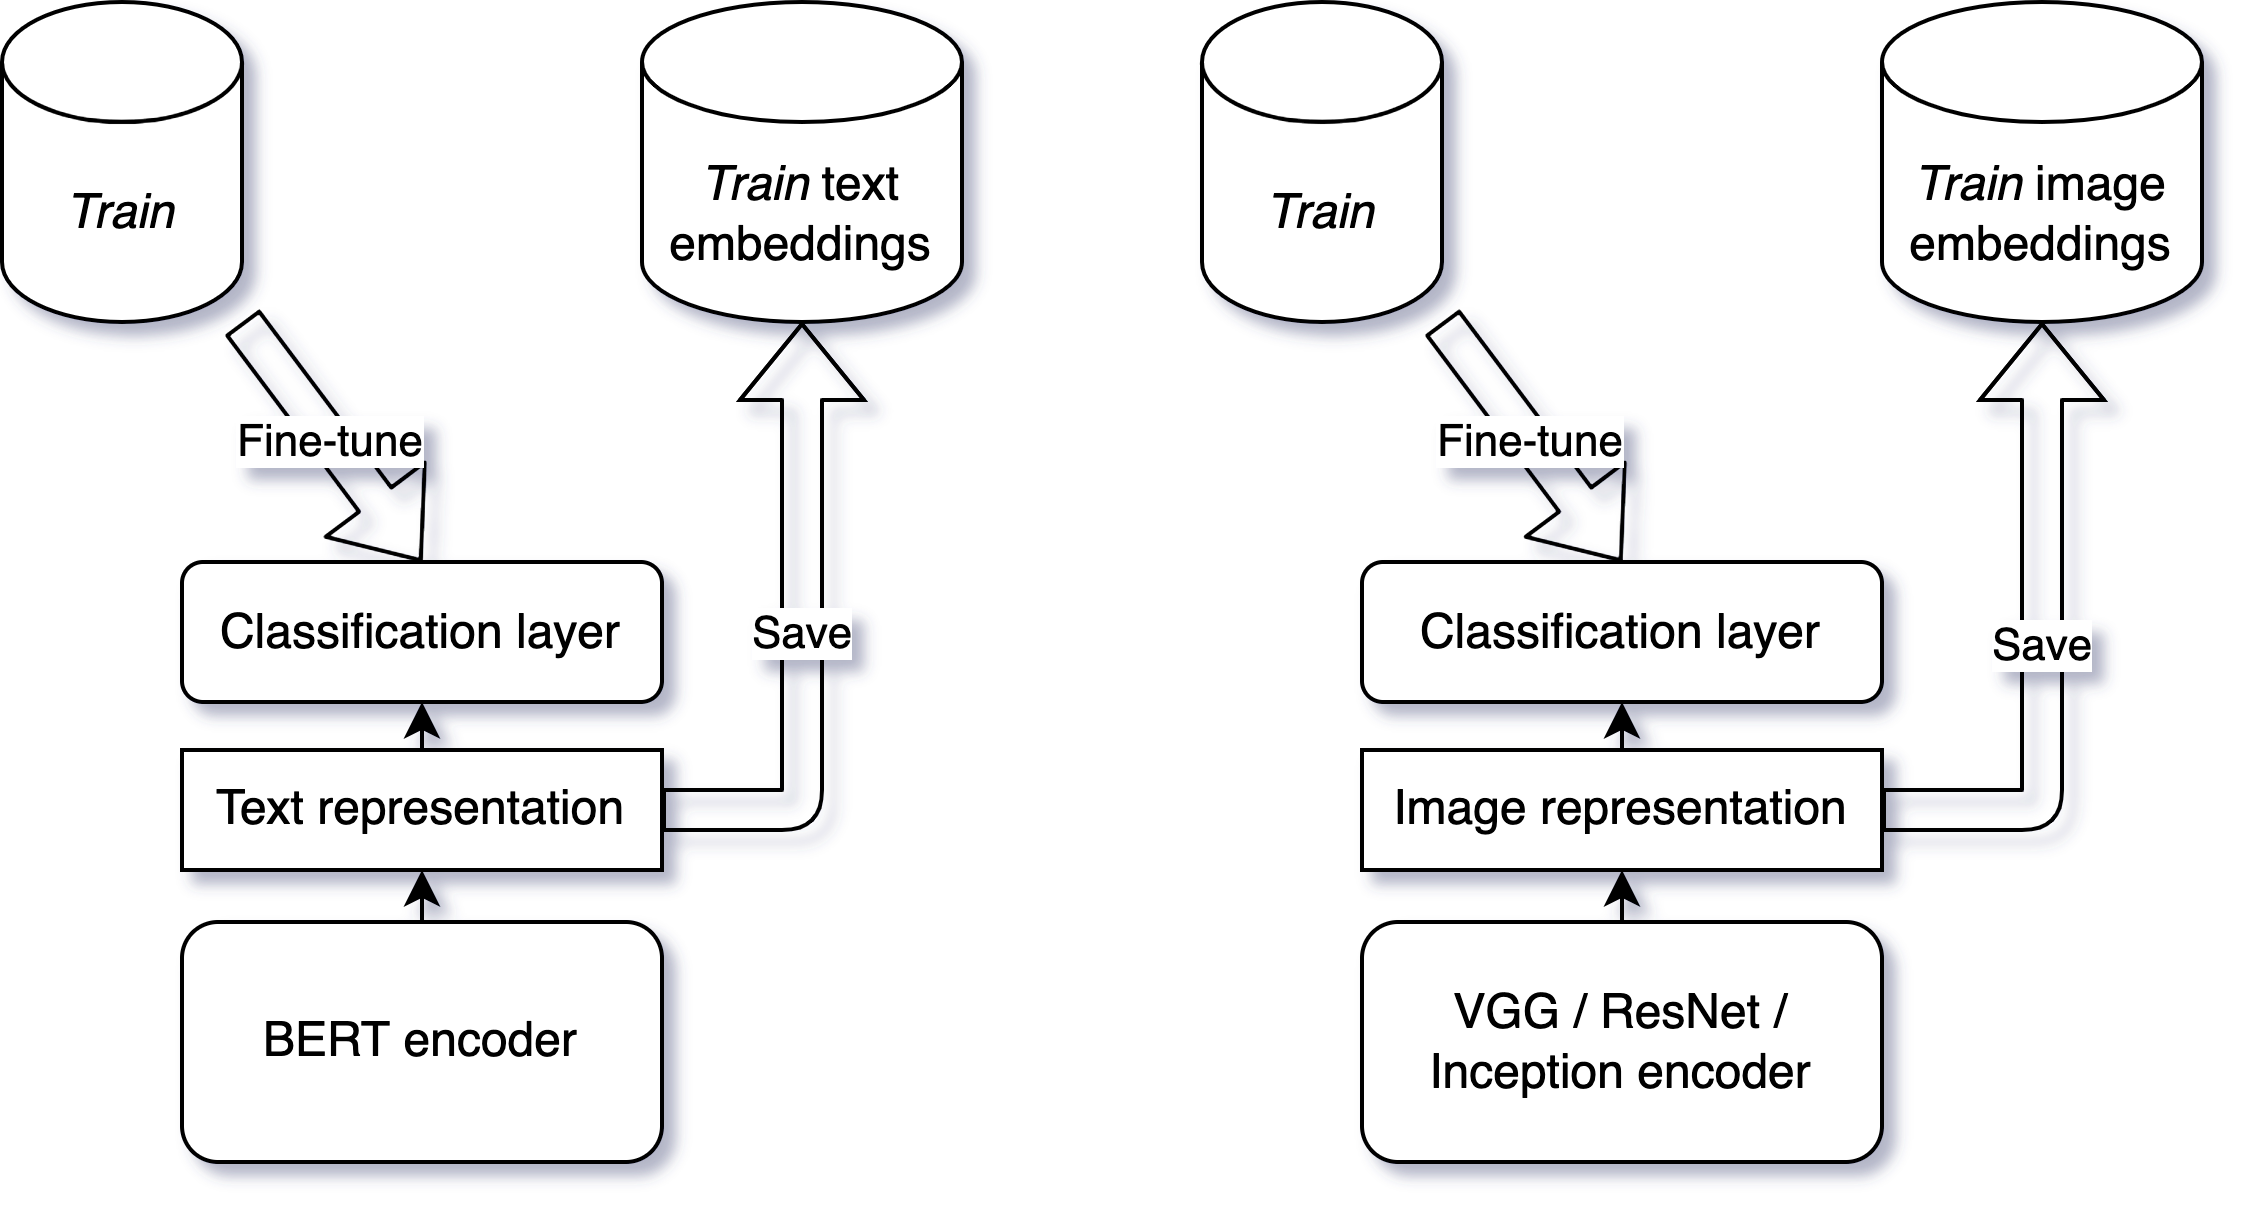
\includegraphics[width=1 \linewidth]{figures/finetune.drawio.png}
  \caption{The first training step is to separately fine-tune the networks via text-classification and image-classification. \textit{Train} denotes a class-disjoint split of either \textit{birds} or \textit{flowers}.}
  \label{fig:fine-tune}
\end{figure}

Next, the classification layers can be removed. Their only purpose was to serve as a proxy for learning the discriminative features of the given domain. The saved embedding of the \textit{train} split are fed into a linear regression model (without regularisation) which finds a projection between them. This is shown in Figure \ref{fig:train}. After this, the image representations (embeddings) can be reached from two directions. Either by using the fine-tuned image encoder, or --- more interestingly --- by taking the description of the image, getting its embedding using the text encoder and then putting that value through the linear regression. This is the core concept we can use for retrieving images using textual descriptions.

\begin{figure}
  \centering
  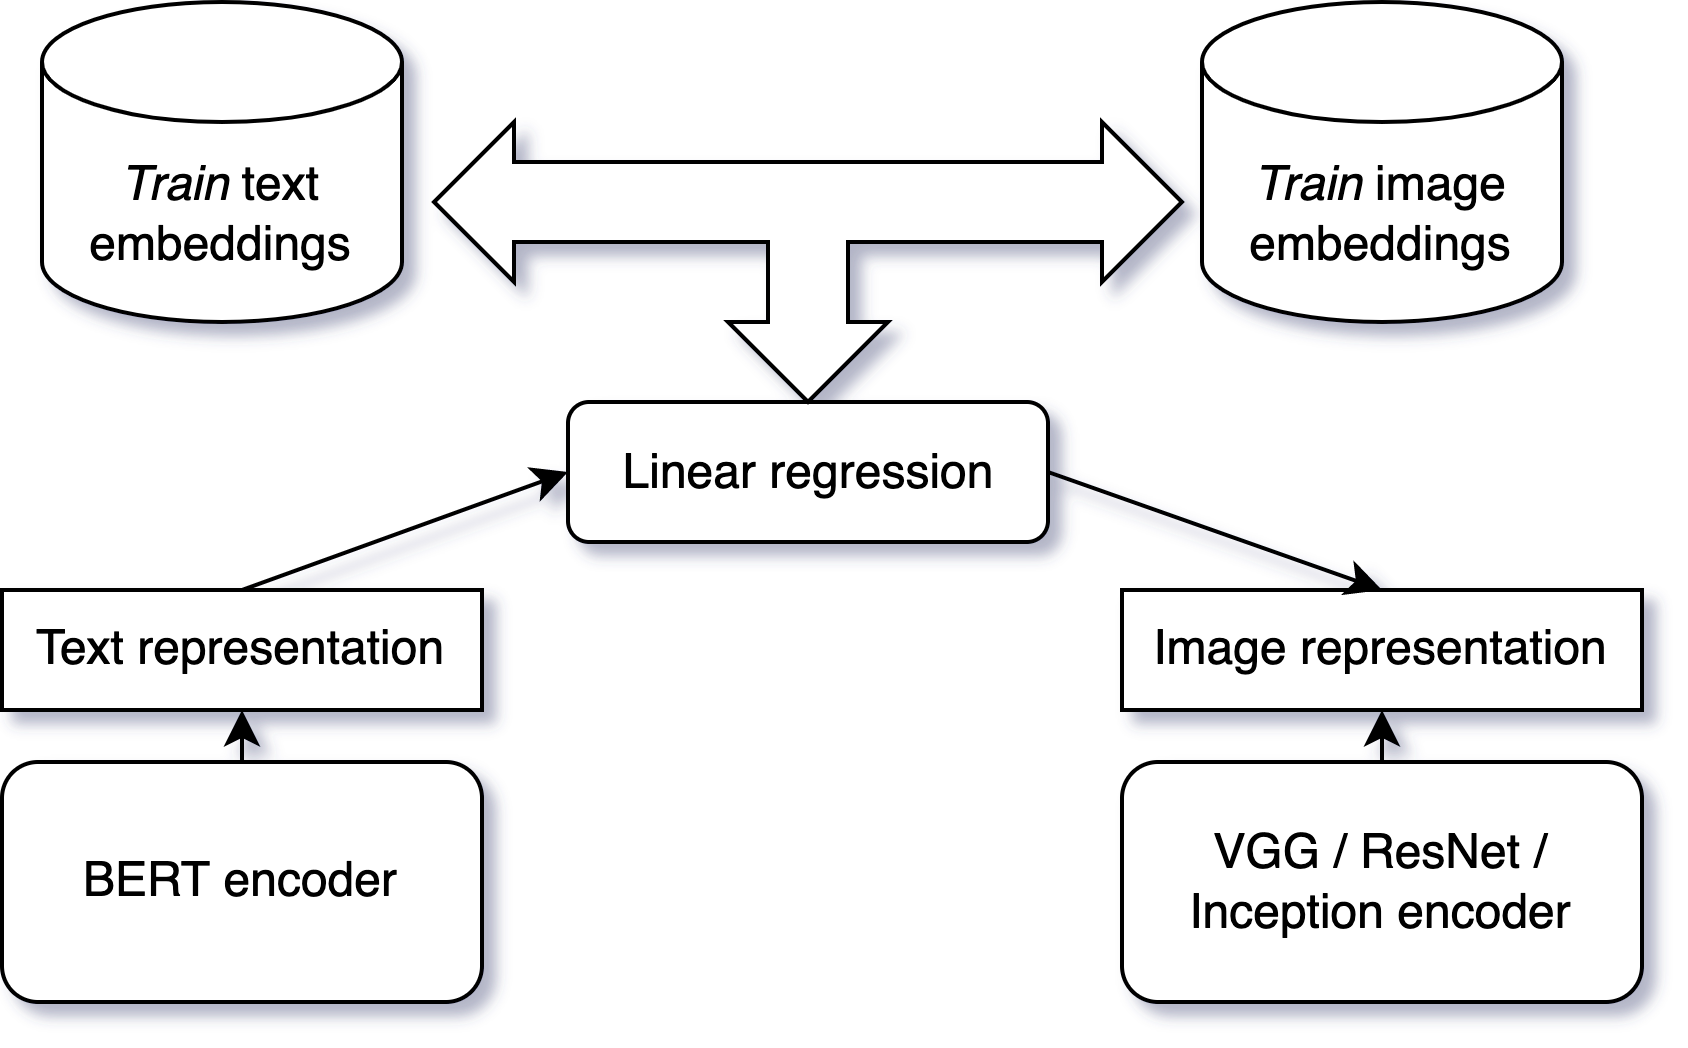
\includegraphics[width=1 \linewidth]{figures/train.drawio.png}
  \caption{For the second-stage of training, the last, classification layers are removed from both models. The exposed, raw text embeddings are mapped to the image-embeddings using a linear projection learned from the actual embeddings of the \textit{train} split.}
  \label{fig:train}
\end{figure}

Figure \ref{fig:evaluate} shows the final step, the system's online operation. The vector representations of the \textit{test} images are calculated and stored in a k-d tree for convenient access. When a new query arrives, it is encoded using the DistilBERT model, the encoding is projected, and the \textit{test} image with the most similar (smallest Euclidean distance) actual image embedding is returned.
\begin{figure}
  \centering
  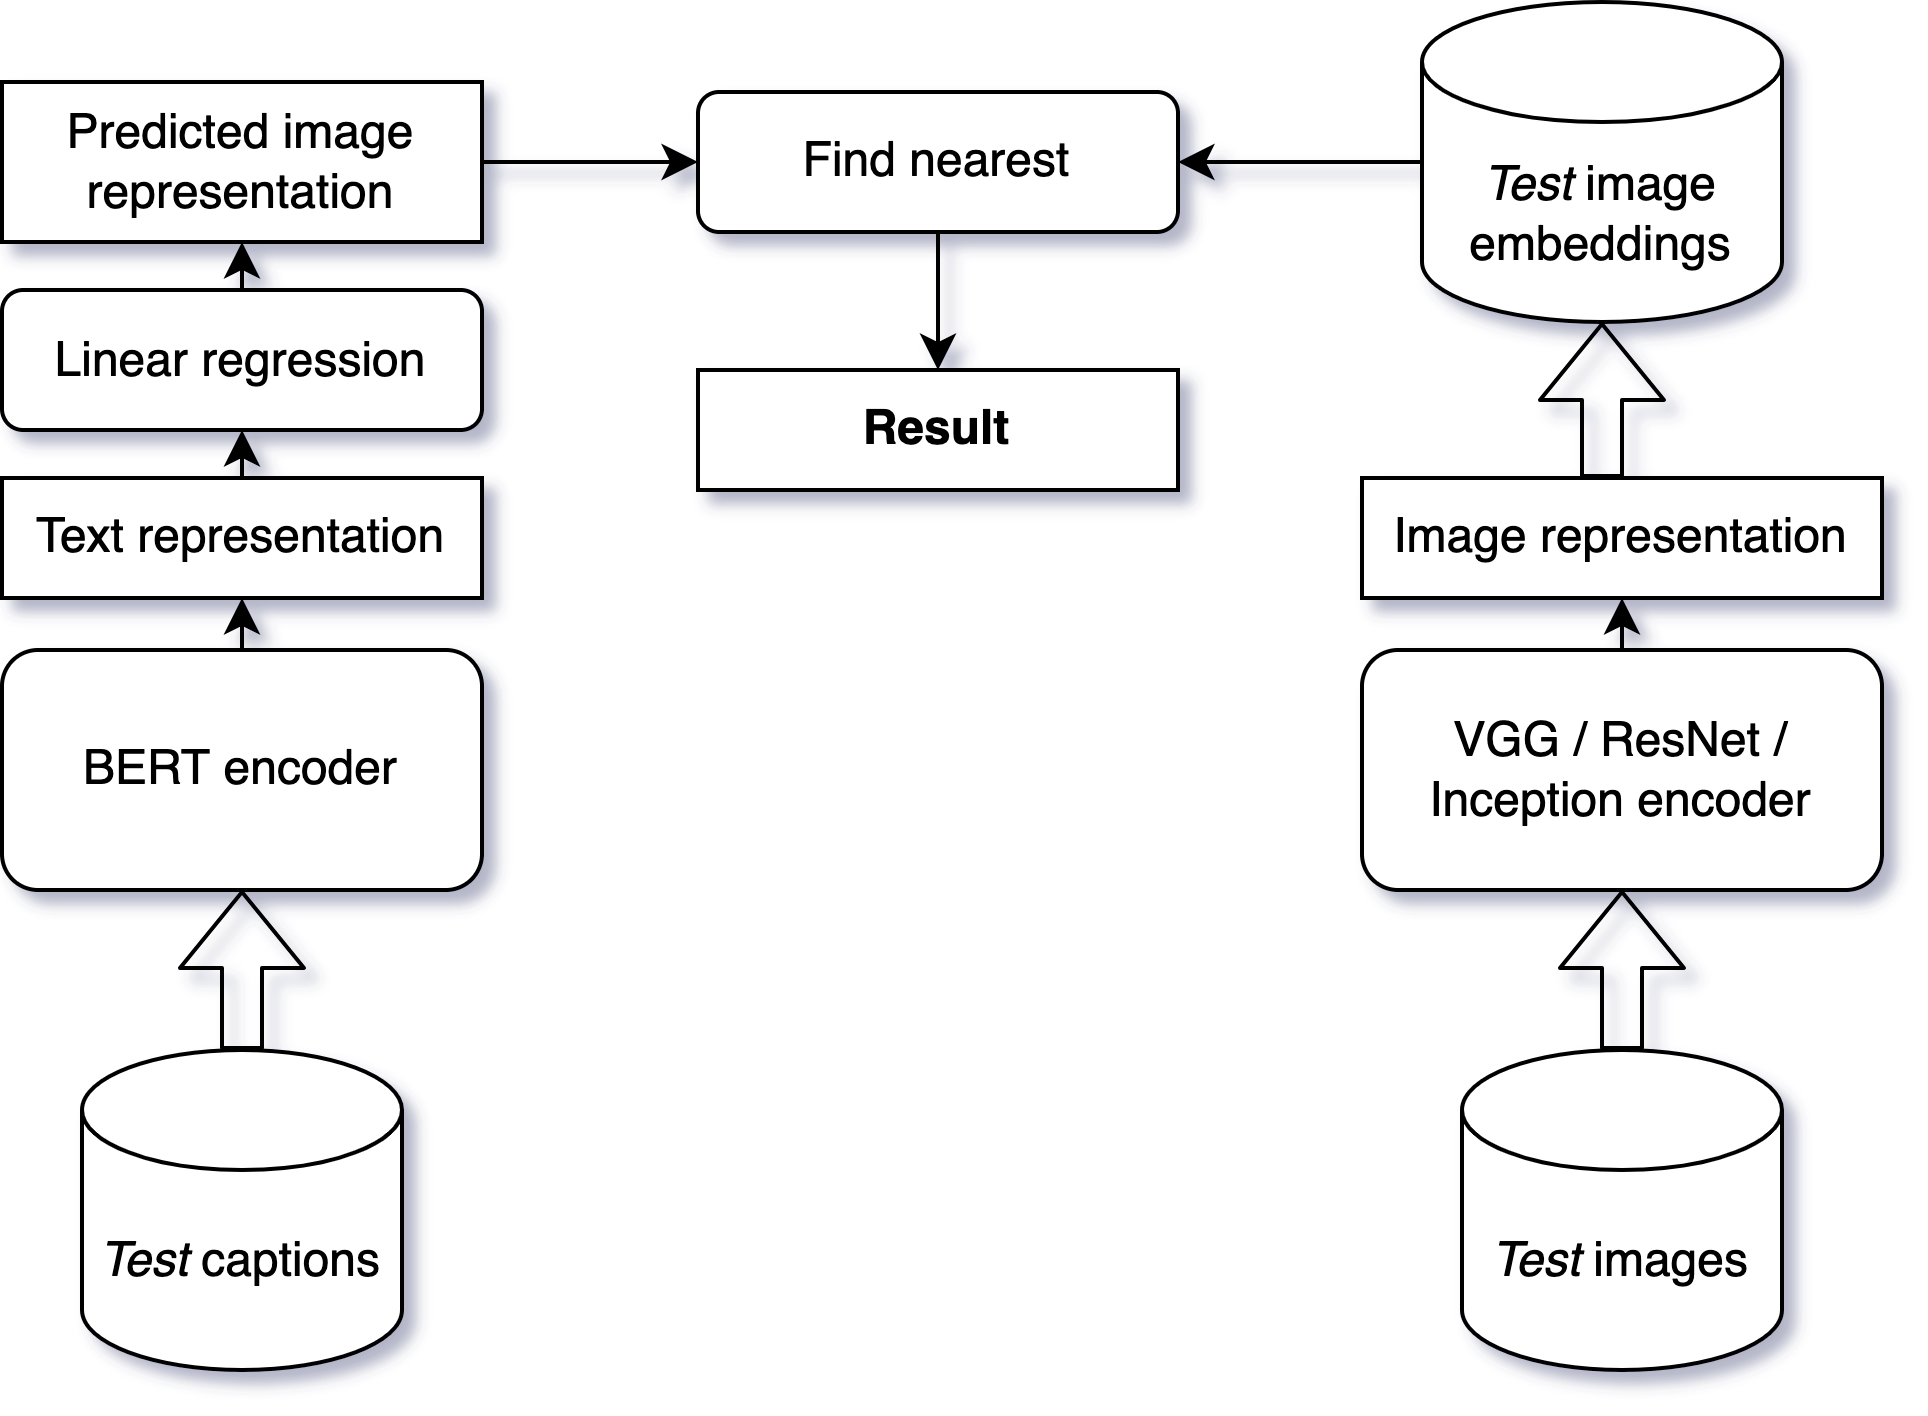
\includegraphics[width=1 \linewidth]{figures/evaluate.drawio.png}
  \caption{First, each image from the \textit{test} split is encoded using the fine-tuned and subsequently beheaded image-classifier. For each caption, an image embedding is predicted using the fine-tuned text encoder and a linear projection. Finally, the images with the most similar embedding to the predicted image embedding are returned.}
  \label{fig:evaluate}
\end{figure}
